\documentclass[tikz, border=1pt]{standalone}
\usepackage{cmap}
\usepackage[T2A]{fontenc}
\usepackage[utf8x]{inputenc}
\usepackage{pgfplots}
\usepackage{pgfplotstable}
\usepackage{xcolor}
\usepackage{amsmath,amssymb}

\usetikzlibrary{decorations.markings, patterns}
\usepgfplotslibrary{fillbetween}

\definecolor{color0}{HTML}{e2431e} % #e2431e
\definecolor{color1}{HTML}{e7711b} % #e7711b
\definecolor{color2}{HTML}{f1ca3a} % #f1ca3a
\definecolor{color3}{HTML}{6f9654} % #6f9654
\definecolor{color4}{HTML}{1c91c0} % #1c91c0
\definecolor{color5}{HTML}{43459d} % #43459d

\tikzset{
	lin/.style={
		line width=0.8pt, 
		mark=none,
		black
	},
}
\begin{document}
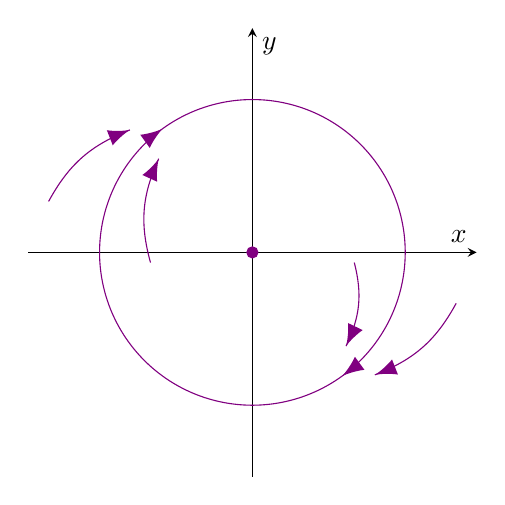
\begin{tikzpicture}
	\begin{axis}[
			axis lines=middle,
			ticks=none,
			xmax=2.2,
			xmin=-2.2,
			ymin=-2.2,
			ymax=2.2,
			xlabel={$x$},
			ylabel={$y$},
			unit vector ratio*=1 1,
		]

		\addplot[
			violet,
			rotate around={90:(0,0)},
			data cs=polar,
			domain=0:360,
			samples=360,
			decoration={
					markings,
					mark=at position 0.1 with {\arrow[scale=-1.5, thick]{latex};},
					mark=at position 0.6 with {\arrow[scale=-1.5, thick]{latex};},
				},
			postaction={decorate},
		] (x,{1.5});

		\draw[fill=violet, violet] (0,0) circle (2pt);
		\draw[violet,decoration={markings,mark=at position 0 with {\arrow[scale=-1.5, rotate=-0,thick]{latex};},},            postaction={decorate}] (45+90:1.3) to[bend left=-20] (axis cs: -1,-0.1);
		\draw[violet,decoration={markings,mark=at position 0 with {\arrow[scale=-1.5, rotate=-0,thick]{latex};},},            postaction={decorate}] (45+90:1.7) to[bend left=-20] (axis cs: -2,0.5);

		\draw[violet,decoration={markings,mark=at position 0 with {\arrow[scale=-1.5, rotate=-0,thick]{latex};},},            postaction={decorate}] (45-90:1.3) to[bend left=-20] (axis cs: 1,-0.1);
		\draw[violet,decoration={markings,mark=at position 0 with {\arrow[scale=-1.5, rotate=-0,thick]{latex};},},            postaction={decorate}] (45-90:1.7) to[bend left=-20] (axis cs: 2,-0.5);

	\end{axis}
\end{tikzpicture}
\end{document}